\documentclass{article}
\usepackage{graphicx} % Required for inserting images

\title{Transformation \& Simulation Methods}
\author{Max Lang}
\date{January 2024}

\begin{document}

\maketitle
\section{Box-Muller algorithm}
\subsection{Intuitive Explanation}

The Box-Muller algorithm is a method for generating normally distributed random numbers from uniformly distributed random numbers. It's a fascinating transformation that bridges the gap between these two types of distributions. Here's an intuitive explanation:

\begin{enumerate}
    \item Start with two independent uniformly distributed random numbers \( U_1 \) and \( U_2 \).
    \item Transform these numbers into polar coordinates. This involves thinking of \( U_1 \) and \( U_2 \) as representing a point in a circle.
    \item Apply specific mathematical functions involving exponentials and trigonometric functions to these polar coordinates.
    \item The transformed numbers now follow a normal distribution, characterized by a higher density of values near the mean.
\end{enumerate}

\subsection{Mathematical Explanation}

Mathematically, the Box-Muller algorithm is expressed through the following steps:

\begin{enumerate}
    \item Start with two independent uniformly distributed random variables \( U_1, U_2 \sim \text{Uniform}(0, 1) \).
    \item Convert to polar coordinates:
    \begin{itemize}
        \item Calculate \( R^2 = -2 \ln(U_1) \)
        \item Calculate \( \Theta = 2\pi U_2 \)
    \end{itemize}
    \item Transform to normally distributed variables:
    \begin{itemize}
        \item Calculate \( Z_0 = \sqrt{-2 \ln(U_1)} \cos(2\pi U_2) \)
        \item Calculate \( Z_1 = \sqrt{-2 \ln(U_1)} \sin(2\pi U_2) \)
    \end{itemize}
\end{enumerate}

These steps convert the uniform distribution of \( U_1 \) and \( U_2 \) into a normal distribution for \( Z_0 \) and \( Z_1 \).
\begin{figure}
    \centering
    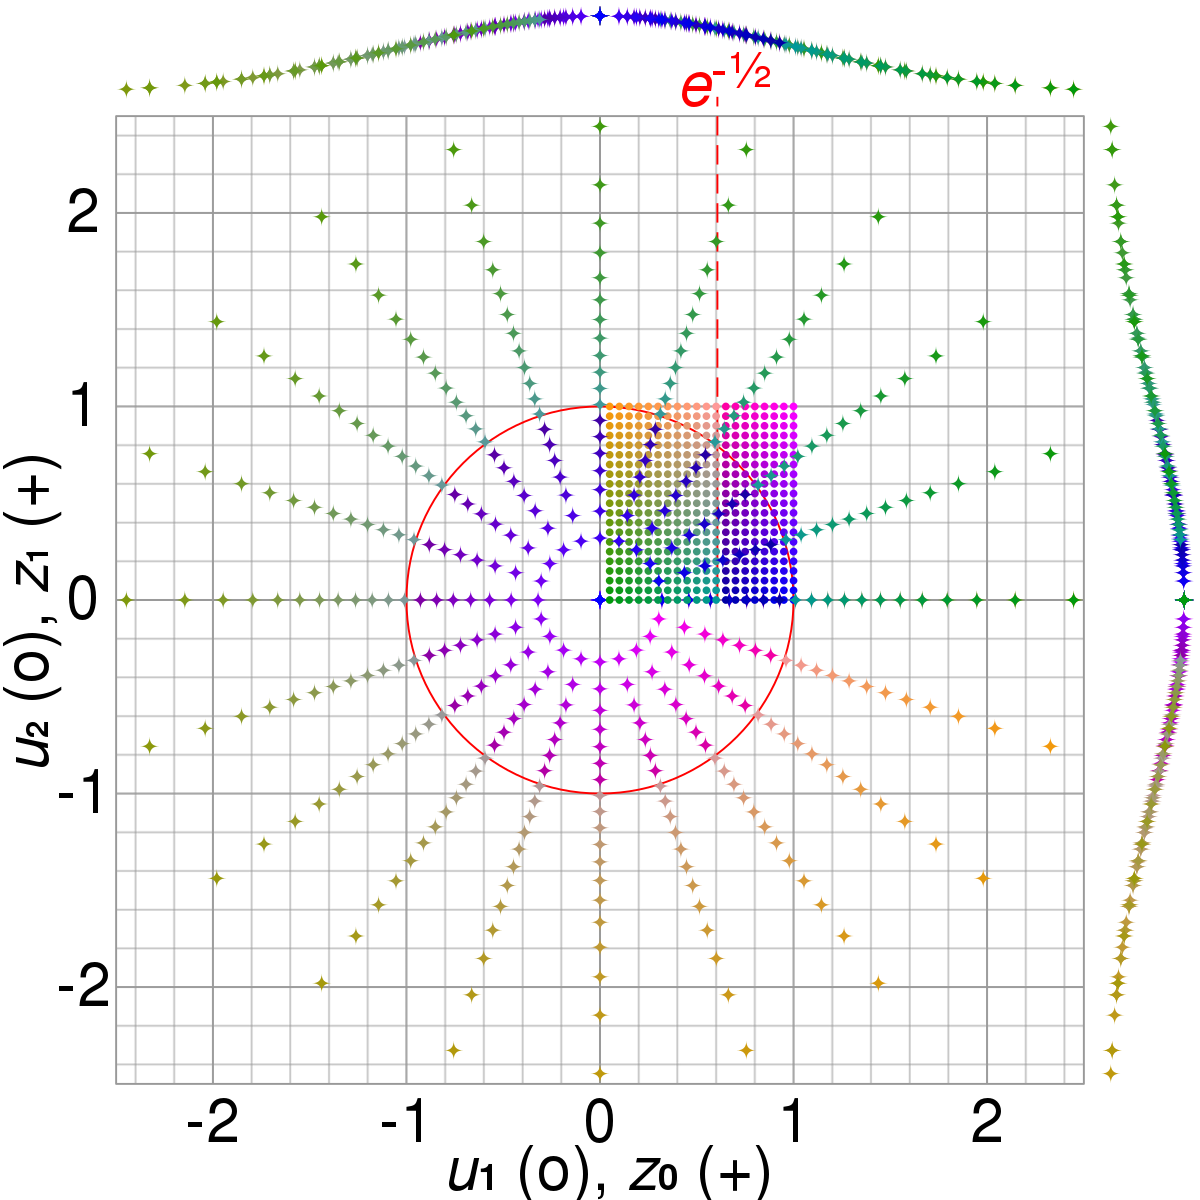
\includegraphics[width=0.5\linewidth]{figures/1200px-Box-Muller_transform_visualisation.svg.png}
    
    
\end{figure}
\begin{figure}
    \centering
    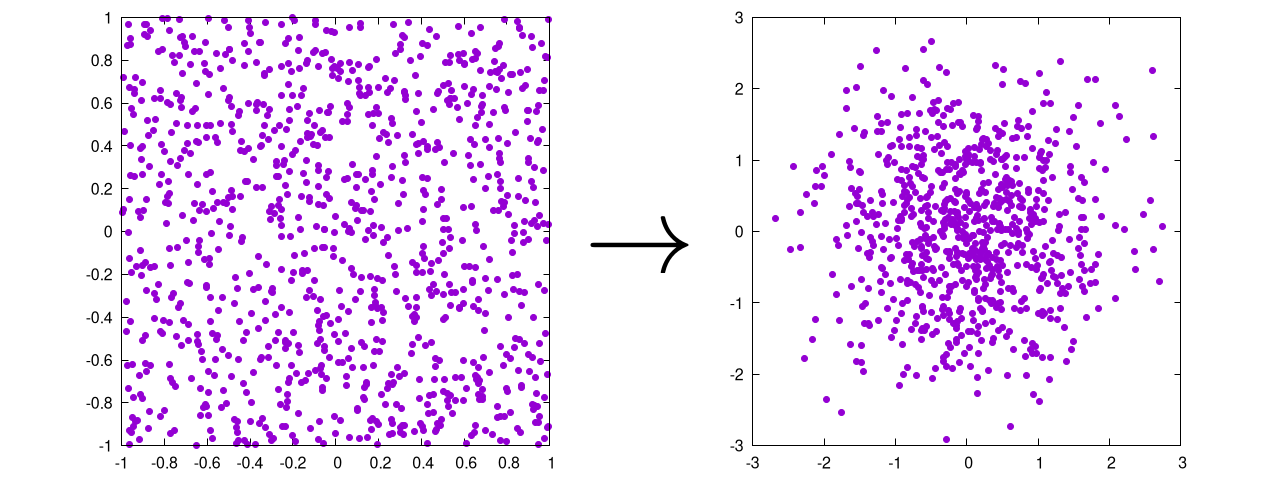
\includegraphics[width=0.75\linewidth]{ox-hilary/simulation-methods/figures/polar_rand_transform.png}
\end{figure}
\begin{figure}
    \centering
    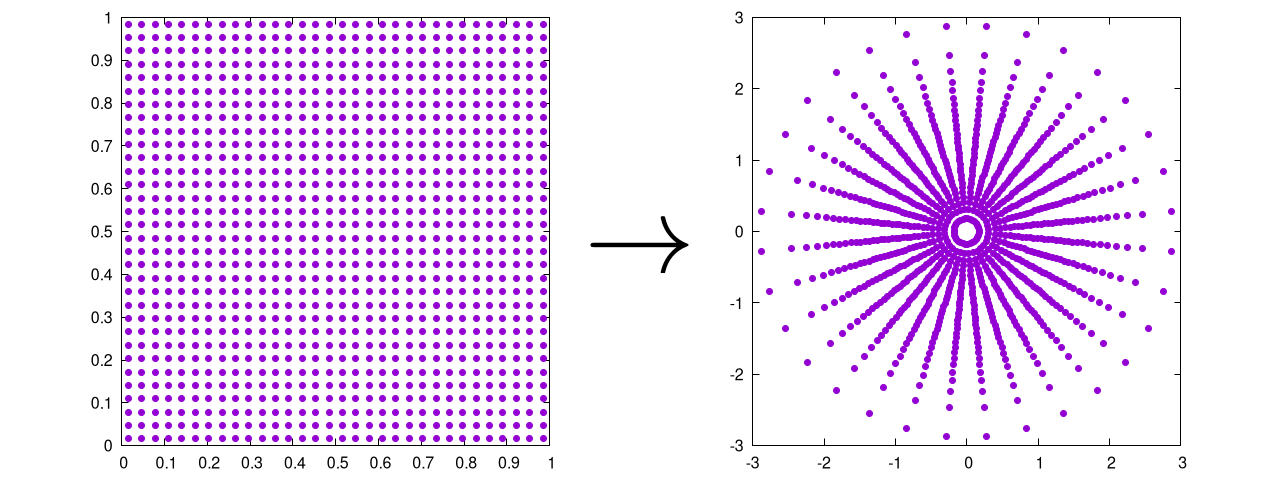
\includegraphics[width=0.75\linewidth]{ox-hilary/simulation-methods/figures/cartesian_grid_transform.png}
\end{figure}
\begin{figure}
    \centering
    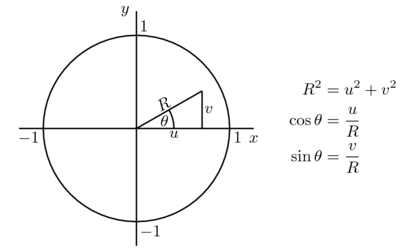
\includegraphics[width=0.75\linewidth]{ox-hilary/simulation-methods/figures/400px-BoxMullerTransformUsingPolarCoordinates.png}
\end{figure}

\section{Sampling via compostion}
\subsection{Intuitive Explanation}
Sampling via composition is a method used to sample from a complex distribution that is made up of several simpler distributions. The idea is similar to building a model out of Lego blocks: instead of trying to carve the entire model out of a single block of plastic (which would be difficult), you assemble it from individual Lego blocks that are easy to handle.

Here's an everyday scenario to understand this better: suppose you're making a sandwich with various ingredients. Each ingredient represents a simpler distribution. You can choose each ingredient (sample from each simpler distribution) independently and then combine them to make your sandwich (the complex distribution). This is essentially what composition is about: combining simpler parts to form a whole.
\begin{enumerate}
    \item Decomposition: Assume you have a joint probability distribution $\pi(x, y)$ that you want to sample from. This joint distribution can often be decomposed into its marginal distribution $\pi(x)$ and conditional distribution $\pi(y \mid x)$.
    \item Sample from Marginal Distribution: First, you sample $x$ from its marginal distribution $\pi(x)$.
    \item Sample from Conditional Distribution: Then, for each sampled $x$, you sample $y$ from the conditional distribution $\pi(y \mid x)$.
\end{enumerate}

By doing this, you obtain a sample $(x, y)$ from the joint distribution $\pi(x, y)$. Mathematically, if $X$ and $Y$ are two random variables with joint distribution $\pi(x, y)$, you can express it as:
$$
\pi(x, y)=\pi(x) \cdot \pi(y \mid x)
$$
where $\pi(x)$ is the probability of $x$ independently, and $\pi(y \mid x)$ is the probability of $y$ given that $x$ has occurred.

This method is particularly useful when it's easier to sample from the marginal and conditional distributions than from the joint distribution directly. It's a divide-and-conquer strategy applied to the problem of sampling from probability distributions.

\section{Rejection sampling}
\subsection{Intuitive Explanation}
The rejection sampling algorithm, also known as acceptance-rejection method, is a basic technique used to generate observations from a distribution. It is particularly useful when direct sampling is difficult. The intuition behind rejection sampling can be understood through a simple analogy:

Imagine you have a dartboard, which represents the probability distribution you want to sample from. However, this dartboard has a complicated shape and is not easy to aim at directly. So instead, you use a larger, rectangular dartboard that completely covers the original one. This rectangle represents a simpler distribution from which you can easily draw samples, often called the proposal distribution.

Now, you throw darts randomly at the larger rectangle. Whenever a dart lands within the bounds of the original complicated dartboard, you accept the throw as a sample from your desired distribution. If the dart lands outside of it but still within the rectangle, you reject it and throw again.

This process ensures that the proportion of accepted darts will represent the complex probability distribution you're interested in, even though you're sampling from a simpler distribution.

\begin{figure}
    \centering
    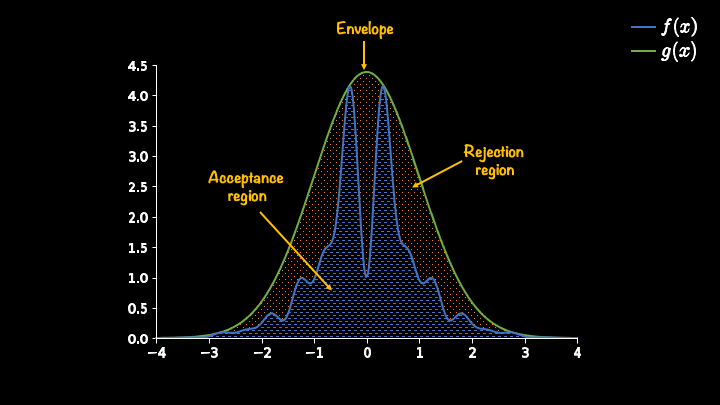
\includegraphics[width=1\linewidth]{ox-hilary/simulation-methods/figures/1_Y8v8ASUKQxeWDHSDTJb7aA.png}
\end{figure}

\subsection{Mathematical Explanation}
Mathematically, rejection sampling follows these steps:
\begin{enumerate}
    \item Choose a Proposal Distribution: Select a proposal distribution, $q(x)$, from which you can easily sample, and a constant $c$ such that $c \cdot q(x)$ is always greater than or equal to your target distribution $p(x)$ for all $x$.
    \item Sample from the Proposal Distribution: Generate a sample, $x$, from $q(x)$.
    \item  Calculate Acceptance Probability: Compute the acceptance probability as $\frac{p(x)}{c \cdot q(x)}$.
    \item Decide to Accept or Reject: Generate a uniform random number, $u$, between 0 and 1 . If $u$ is less than or equal to the acceptance probability, accept $x$ as a sample from $p(x)$; otherwise, reject $x$.
    \item  Repeat: Continue this process until you have enough accepted samples.
\end{enumerate}

This algorithm leverages the fact that scaling up the proposal distribution and then selectively accepting samples can simulate the more complicated target distribution. The constant $c$ ensures that the scaled-up proposal distribution always encompasses the target distribution, making sure that every part of the target distribution has a chance to be sampled. The acceptance probability corrects for the areas where the proposal distribution is too large, leading to an accurate representation of the target distribution.

\subsection{Algorithm}

Given two densities $\pi, q$ on $\mathrm{X}$ with $\pi(x) \leq M q(x)$ for all $x \in \mathbb{X}$ and some $M<\infty$, we can generate a sample from $\pi$ as follows:
\newline
1. Draw $X \sim q$.
\newline
2. Accept $X=x$ as a sample from $\pi$ with probability
$$
\alpha=\frac{\pi(x)}{M \cdot q(x)},
$$
otherwise go back to step 1 .
\newline
Note that to implement rejection sampling, we need to implement a mechanism to either "do this" or "do that" according to some probability $\alpha \in[0,1]$. The standard way to implement this goes as follows.\newline
\newline
1. Draw $U \sim \mathcal{U}_{[0,1]}$. \newline
2. If $U \leq \alpha$ then "do this", otherwise "do that".
\newline
Indeed $\mathbb{P}(U \leq \alpha)=\alpha$ when $U \sim \mathcal{U}_{[0,1]}$, so that the above scheme will "do this" with probability $\alpha$.

\end{document}
